% Chapter Template

\chapter{Experimental Results on Routing Strategies} % Main chapter title

\label{expereince}

\lhead{Chapter 2. \emph{Experimental Results on Routing Strategies}}

\section{Experiment Test Setup}
We tested our experiments on clusters of cisco's server with linux containers with different configuration set ups on Lurch. In the case of needs, dynamic modifications also have been added on Lurch to be more interactive for different test scnearios.

In this chapter we will show, test and validate our 4 routing strategies on 2 different setup networks with 5 nodes (medium size) and another one with 17 nodes (large size) each one with costumized capacity. We plot rates in Kbps vs time for each link involved in strategy. $\{ai\}$, $i=$1:8 are Access Points and nodes with \textit{NodeID} are Autonomous nodes in the network.
   
In all scenarios we plot the figures of each link by nodeID of ends connected. In, Out means the direction of packets that come to node. We consider number of hops as cost of link as it is meaningful in ICN architecture.
\textit{TreeOnConsumer}, \textit{TreeOnProducer}, \textit{MinCostMultipath}, \textit{MaxFlow} are 4 different parameters of RoutingNDN module to choose which are done for \textit{Medium} and \textit{Large} size. We have put the result of each case inside the subsection.

In all cases Clients are searching /n/a/noseg chunk and repositories are containing /n folder which has alphabetical letters to like a,b,c,d, ... then chunks of \textit{BigBuckBunny.mp4} are appended to them. Engine of repository is an application called \textit{repo-ng}. 

\section{Strategies on Medium Size NDN Network}


\subsection{TreeOnConsumer}
As figure \ref{TreeOnConsumer} shows, 'luca' and 'jordan' nodes are clients searching '/n/a/noseg' chunk and 'shahab' node is producer of content. The first prefix of content is /n folder contains.

Figure \ref{treeonconsumer} shows 4 traced rates in which yellow and green one are data packets. Same packets are routed through \textit{TreeOnConsumer} tree to the clients with different rates. In this figure you can see the delay between 'sj' and 'sl' which is becasue of capacity difference of between containers. So you have 2 threads on 2 different machines occuring and recorded at the same time.

\begin{figure}[H]

\begin{center}

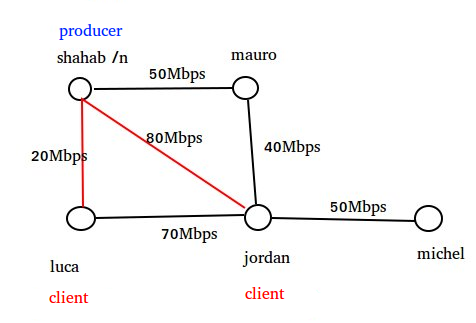
\includegraphics[scale = 0.4]{Figures/TreeOnConsumer.png}

\caption{TreeOnConsumer Tree Medium} \label{TreeOnConsumer} 


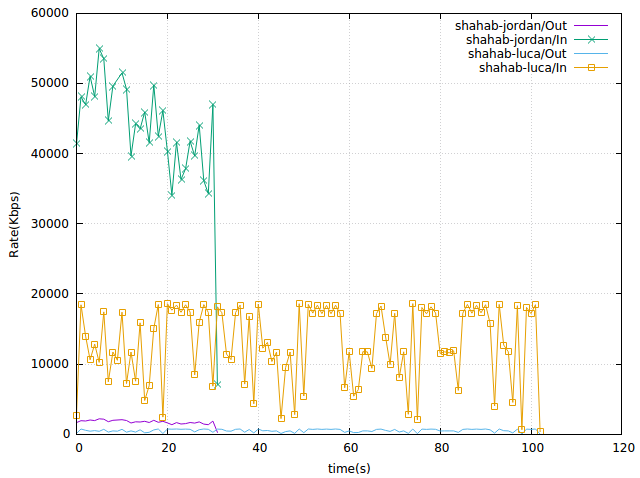
\includegraphics[scale = 0.4]{Figures/treeonconsumer.png}

\caption{TreeOnConsumer (Rate vs Time) Medium} \label{treeonconsumer} 


\end{center}

\end{figure}


\subsection{TreeOnProducer}
Figure \ref{TreeOnProducer} shows 'jordan', a client who searches '/n/a/noseg' and 2 producers ('shahab','mauro') who send packets to client by this strategy using tree of \textit{TreeOnProducer}. 
Figure \ref{treeonproducer} shows as well this downloading traced during time which can be used whenever client wants a high quality content.
\begin{figure}[H]

\begin{center}

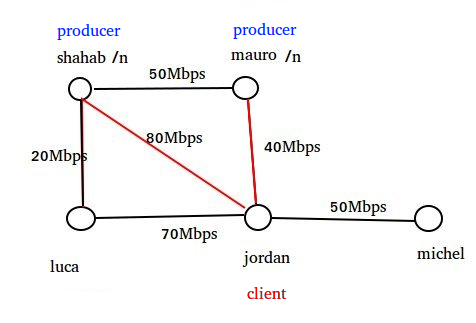
\includegraphics[scale = 0.4]{Figures/TreeOnProducer.png}

\caption{TreeOnProducer Tree Medium} \label{TreeOnProducer} 


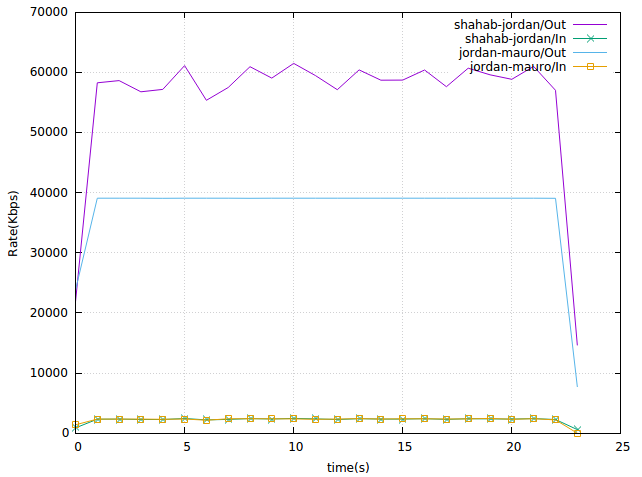
\includegraphics[scale = 0.4]{Figures/treeonproducer.png}

\caption{TreeOnProducer (Rate vs Time) Medium} \label{treeonproducer} 


\end{center}

\end{figure}

\subsection{MinCostMultipath}
Figure \ref{MinCostMultipath} shows \textit{MinCostMultipath} tree of minimum of network in which we use number of hops as cost of links. This is the case in which we want to broadcast video livestreaming as we discussed. Same chunk of datas are searching at the same time for a live movie like a football match content to all clients.
 
Figure \ref{mincost} shows traced data as well.
\begin{figure}[H]

\begin{center}

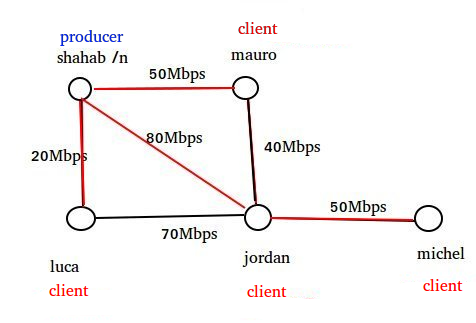
\includegraphics[scale = 0.4]{Figures/MinCostMultipath.png}

\caption{MinCostMultipath Tree Medium} \label{MinCostMultipath} 

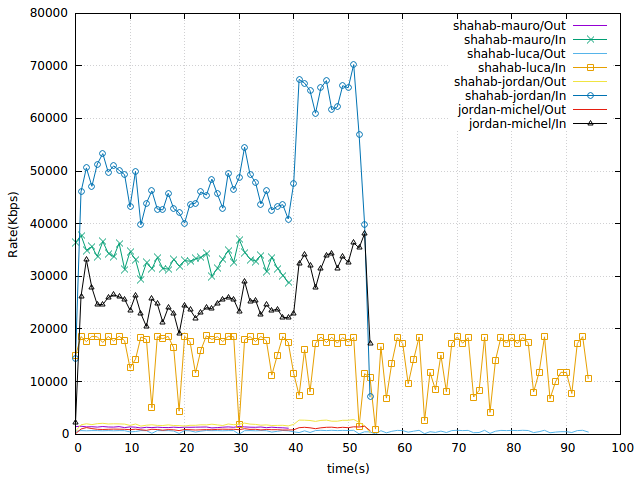
\includegraphics[scale = 0.4]{Figures/mincostmultipath.png}
\caption{MinCostMultipath (Rate vs Time) Medium} \label{mincost} 

\end{center}

\end{figure}

\subsection{MaxFlow}
In figure \ref{MaxFlow} 'jordan' node gets information from all of path possible to maximize data throughput.

Figure \ref{maxflow} shows data rates which are maximum for each link. It can be used whenever clients need higher quality data.

You can see for marginal paths you have on the stable rates.
\begin{figure}[H]

\begin{center}

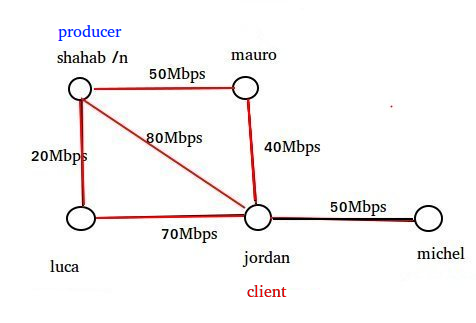
\includegraphics[scale = 0.4]{Figures/MaxFlow.png}

\caption{MaxFlow Medium} \label{MaxFlow} 


\end{center}

\end{figure}

\begin{figure}[H]

\begin{center}

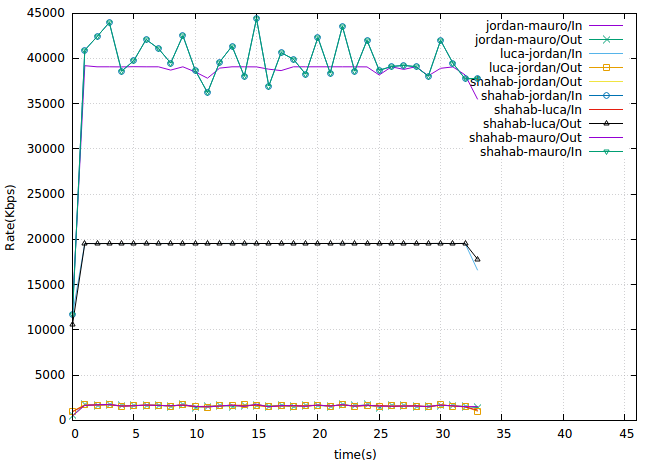
\includegraphics[scale = 0.4]{Figures/maxflow.png}

\caption{MaxFlow (Rate vs Time(s)) Medium} \label{maxflow} 


\end{center}

\end{figure}




 

\section{Strategies on Large Size NDN Network}

\subsection{TreeOnConsumer}
Figure \ref{TreeOnConsumer_big} shows a red subgraph, $a1, a2, a3, a4$ are Acces Points on which the mobile clients are connected through \textit{TreeOnConsumer} tree on the network.\\
In \ref{treeonconsumer_big}  rates are traced against time as well. The 'sj' link curve is upper than the other becasue you have 3 clients Child on this side against 'sg' side in which you have just one Child. So the Interest/Data packets are bigger on right first depth of tree.

\begin{figure}[H]

\begin{center}

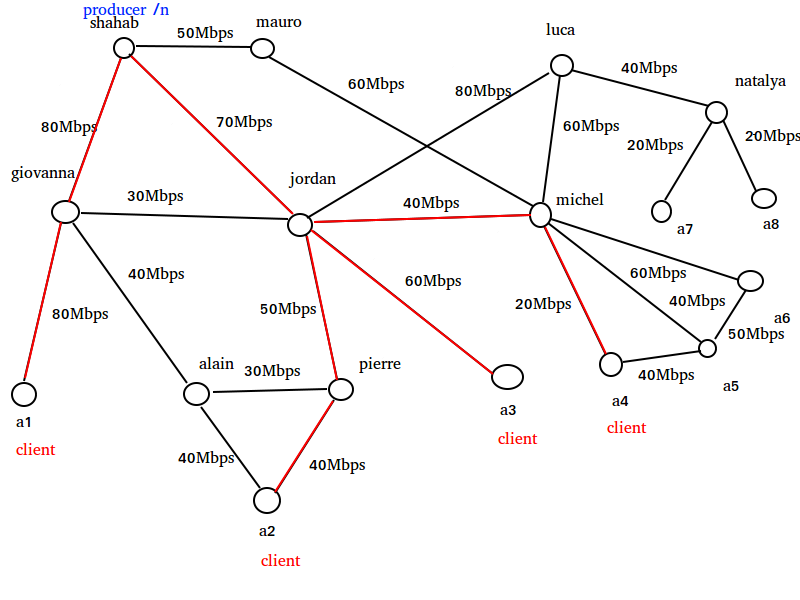
\includegraphics[scale = 0.4]{Figures/TreeOnConsumer_big.png}

\caption{TreeOnConsumer Tree Large} \label{TreeOnConsumer_big} 


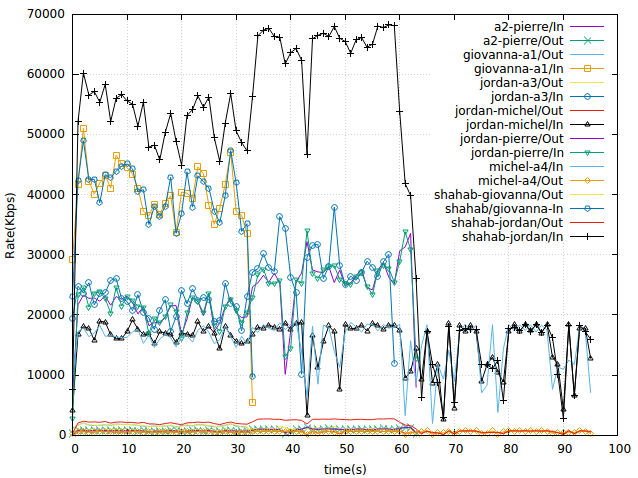
\includegraphics[scale = 0.4]{Figures/treeonconsumer_big.png}

\caption{TreeOnConsumer (Rate vs Time) Large} \label{treeonconsumer_big} 


\end{center}

\end{figure}


Figure \ref{Mob1} shows the first step of client mobility in which the mobile station is attached to node $n10$. Figure \ref{mob1} shows also the Interest/Data packets which are going through shortest paths.

You can see in figure \ref{Mo2} that as soon as mobile client is attached to $n11$ routing update is happened and new routing is traced.

Same case for \ref{Mob3} which is for showing that update can occured. This update can be designed periodically or to have an algorithm. After we need to know more practical constraints like how much time takes that an routing update happens? The answer depends on what we use for engine forwarder and its implementations. 



\begin{figure}[H]

\begin{center}

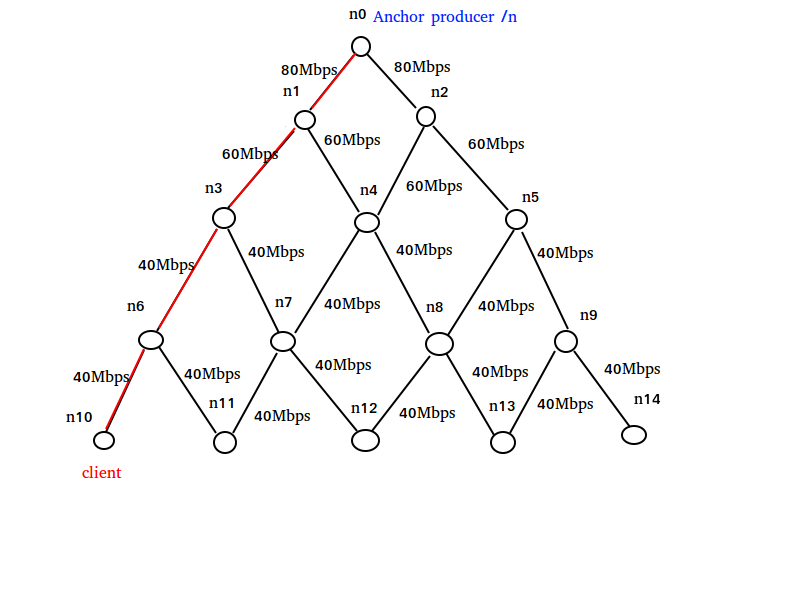
\includegraphics[scale = 0.4]{Figures/Mob1.png}

\caption{TreeOnConsumer Mobility Large} \label{Mob1} 


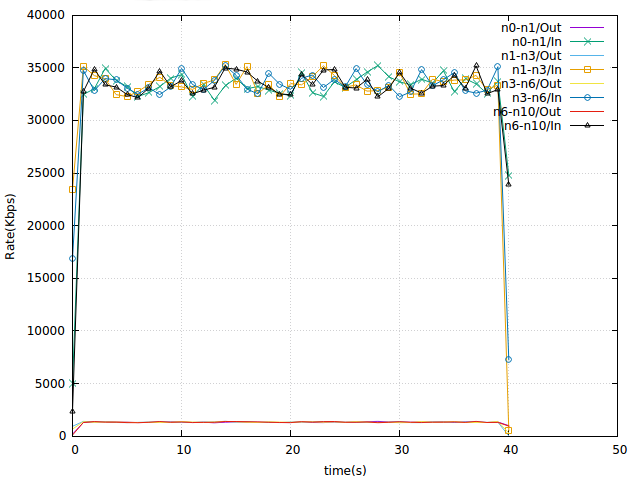
\includegraphics[scale = 0.4]{Figures/mob1.png}

\caption{TreeOnConsumer Mobility (Rate vs Time) Large} \label{mob1} 


\end{center}

\end{figure}

\begin{figure}[H]

\begin{center}

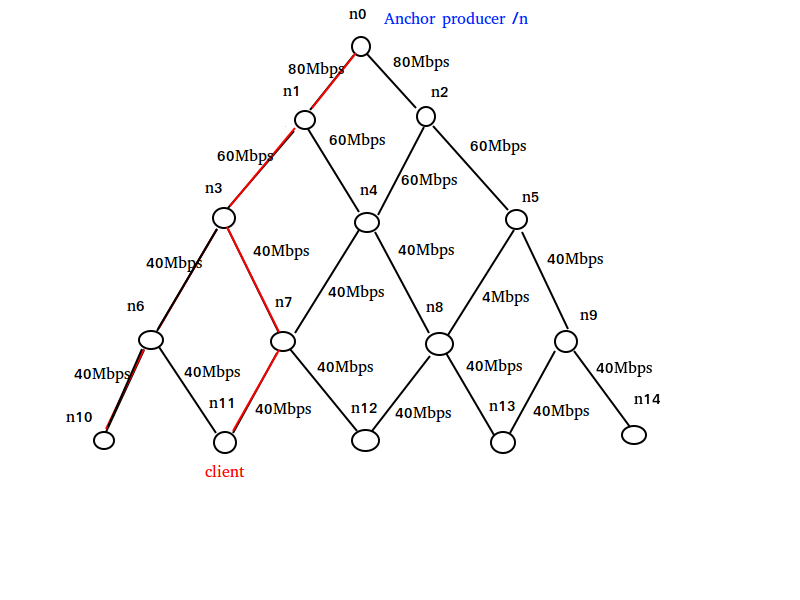
\includegraphics[scale = 0.4]{Figures/Mob2.png}

\caption{TreeOnConsumer Mobility Large} \label{Mob2} 


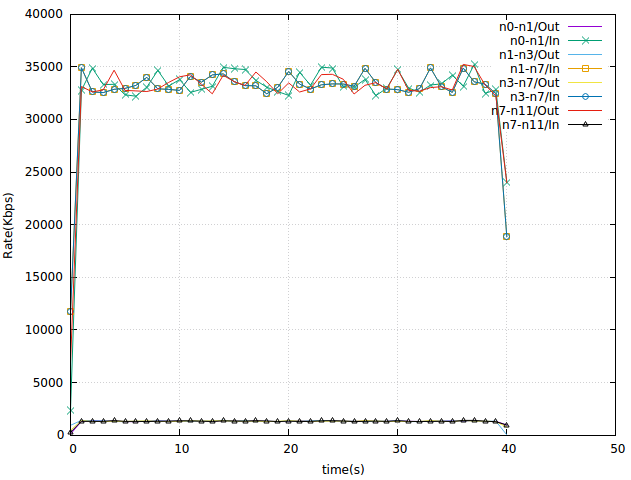
\includegraphics[scale = 0.4]{Figures/mob2.png}

\caption{TreeOnConsumer Mobility (Rate vs Time) Large} \label{mob2} 


\end{center}

\end{figure}

\begin{figure}[H]

\begin{center}

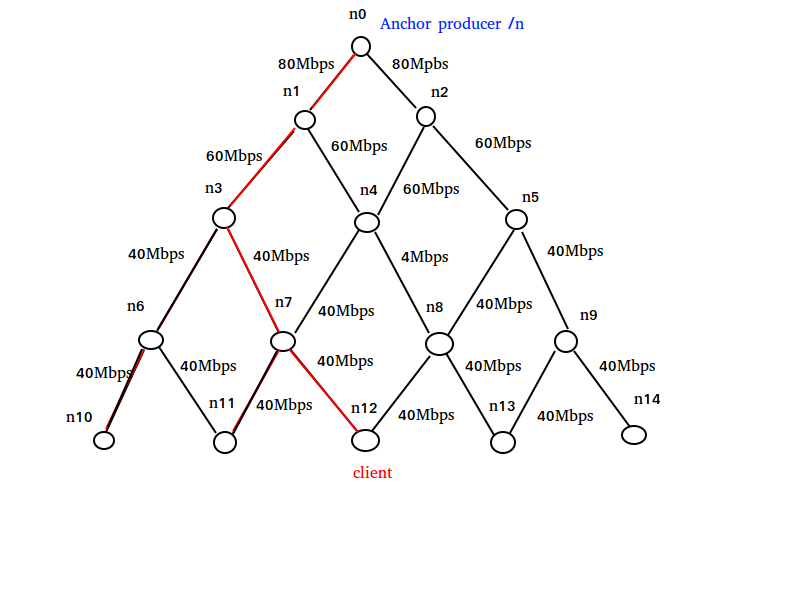
\includegraphics[scale = 0.4]{Figures/Mob3.png}

\caption{TreeOnConsumer Mobility Large} \label{Mob3} 


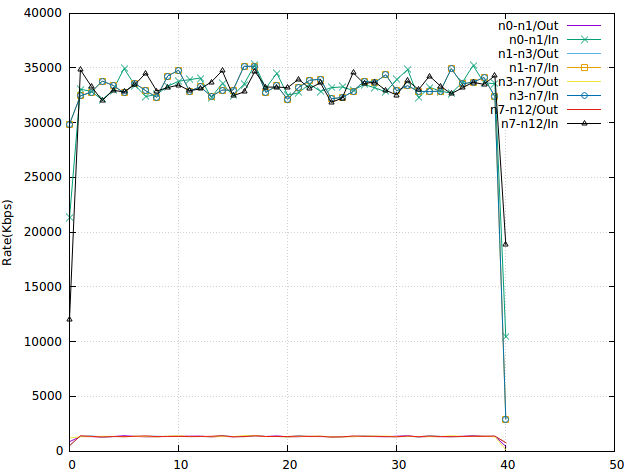
\includegraphics[scale = 0.4]{Figures/mob3.png}

\caption{TreeOnConsumer Mobility (Rate vs Time) Large} \label{mob3} 


\end{center}

\end{figure}





\subsection{TreeOnProducer}
Figure \ref{TreeOnProducer_big} shows $a6$ as Access Point client which recieves data from different producer nodes at the same time.

This strategy can be used whenever client can achieve to multiple repositories and it can download his chunk at the same time.

\begin{figure}[H]

\begin{center}

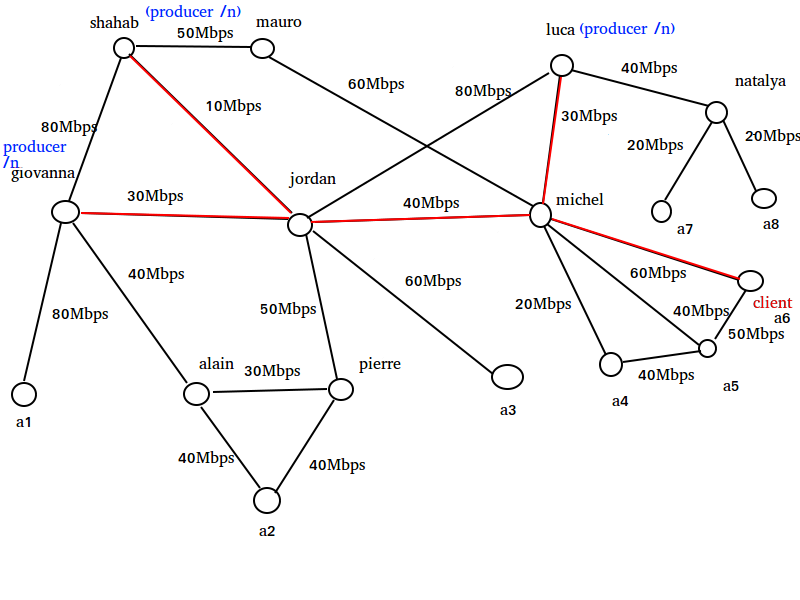
\includegraphics[scale = 0.4]{Figures/TreeOnProducer_big.png}

\caption{TreeOnProducer Tree Medium} \label{TreeOnProducer_big} 


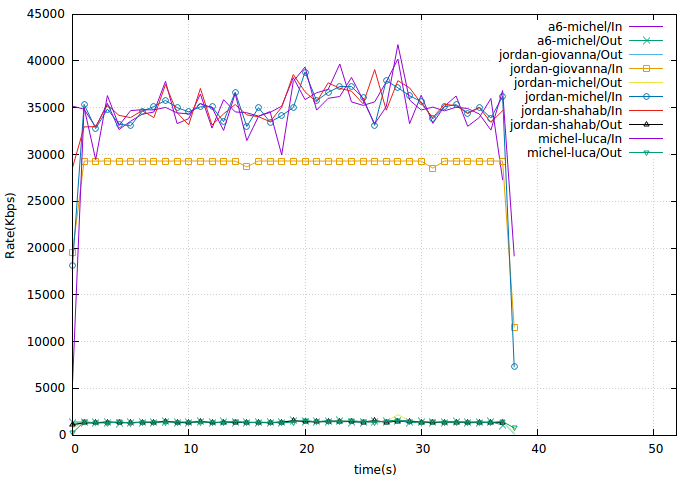
\includegraphics[scale = 0.4]{Figures/treeonproducer_big.png}

\caption{TreeOnProducer (Rate vs Time) Large} \label{treeonproducer_big} 


\end{center}

\end{figure}


\subsection{MinCostMultipath}
Figure \ref{MinCostMultiPath} shows how the \textit{MinCostmultiPath} tree is chosen to deliver content to all clients which are connected to access points.
 
Notably this strategy can be used when you want to do a \textit{Equal Cost Multi Path} (ECMP) routing in which your minimized paths have equal cost to destination so we should use load-balance or multipath forwading strategy to allow traffic to pass along the network. 

The algorithm of this strategy is written by the idea of searching minimum multipath from producer to client.

\begin{figure}[H]

\begin{center}

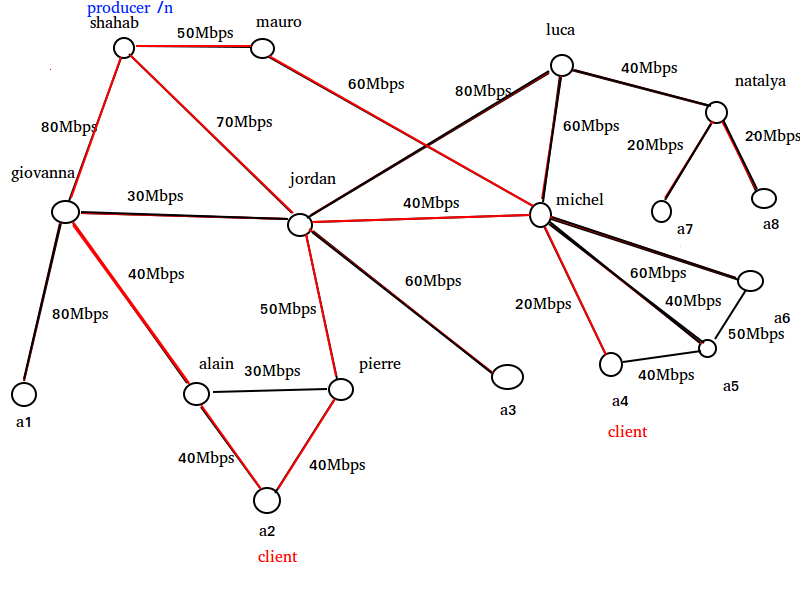
\includegraphics[scale = 0.4]{Figures/MinCostMultipath_big.png}

\caption{MinCostMultiPath Tree Large} \label{MinCostMultiPath} 


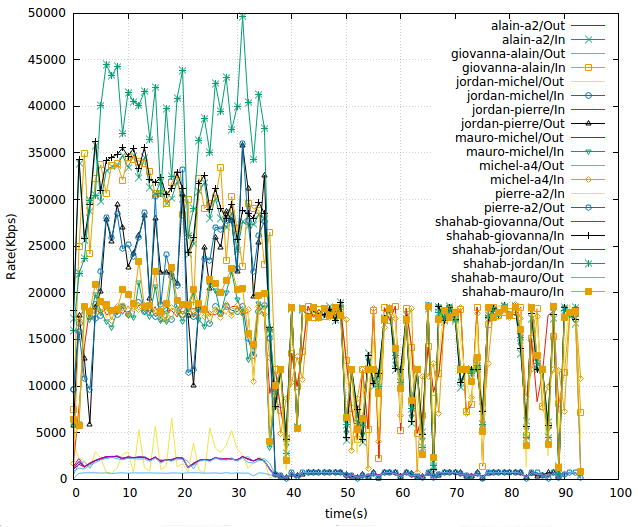
\includegraphics[scale = 0.4]{Figures/mincostmultipath_big.png}

\caption{MinCostMultiPath (Rate vs Time) Large} \label{mincostmultipath} 


\end{center}

\end{figure}


\textbf{\Large{Multi Consumers and Producers}}. Figure \ref{Multi-Repo-Client} as you can see we can have $n$ producers and $m$ consumers want to download at the same time. This strategy chooses the shortest paths between clients and consumers using to give routes update. Actually for each consumer, algorithm looks which producer is closer using \textit{shortest path} then set routes properly. This strategy can be very usefull in ICN networks becasue of its architecture. 

Routing is the core issues of any network even Network of streets and broadways! It's the idea of Routing in general is to have knowledge about network and its proper graph then have a table at each router to calculate best routes for each packet. This table can be static or dynamic, normally in practice routers are dynamic in function of network needs. 

One beautiful idea which is very \textit{à la mode} in research and development in these days becasue of its advantages is to have a \textbf{S}oftware \textbf{D}efine \textbf{N}etwork. The SDN can be a central controller who allows users to modify the network in terms of capacities, network topology, routing, and whatever you can think about the network which can be changes dynamically.

You can also imagine a scenario to occur, you can have algorithms inside algorithms to run full automate evidences. This strategy can be very usefull in these scnearios becasue of NDN architecutre.

By running this strategy on Lurch, it can understand whenever you want to do a ECMP or Multi repository client. It's important becasue network when you have your controller (Lurch) who understands the scenario in which you want to apply your strategies. 

  


\begin{figure}[H]

\begin{center}


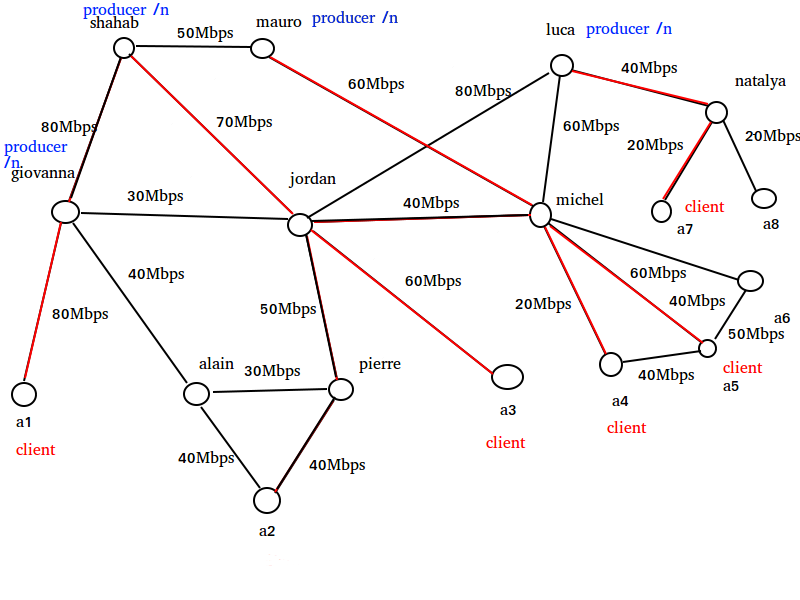
\includegraphics[scale = 0.4]{Figures/Multi-Repo-Client.png}

\caption{Multi Consumers and Producers Large} \label{Multi-Repo-Client} 


\end{center}

\end{figure}




\begin{figure}[H]

\begin{center}


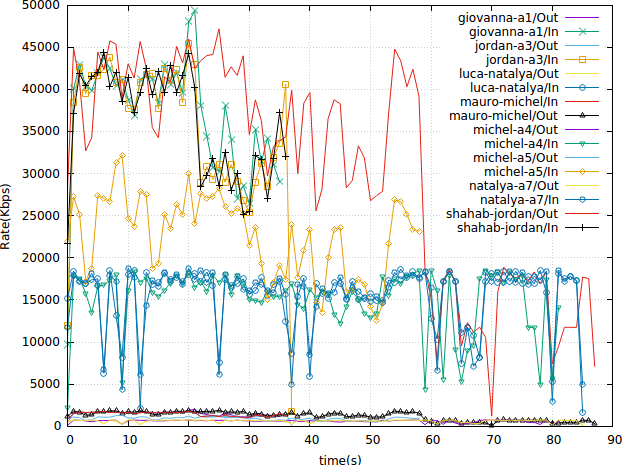
\includegraphics[scale = 0.4]{Figures/multi-repo-client.png}

\caption{Multi Consumers and Producers (Rate vs Time) Large} \label{multi-repo-client} 


\end{center}

\end{figure}

Now let's consider an interesting point of this strategy in Mobility of ICN. Figure \ref{Step1} shows the first step of a mobility scenario in which producer is attached to n18. In this case producer can be a Robot carrying a webcam to capture a film from environment send it to network as the content producer. The clients are mobile stations and are attached to base stations as well.   


\begin{figure}[H]

\begin{center}


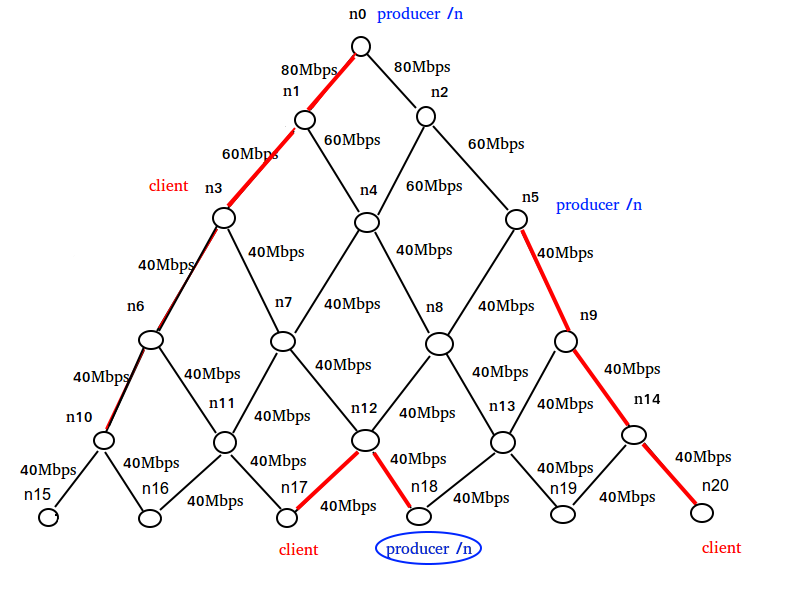
\includegraphics[scale = 0.4]{Figures/Step1.png}

\caption{Producer Mobility step 1 Large} \label{Step1} 

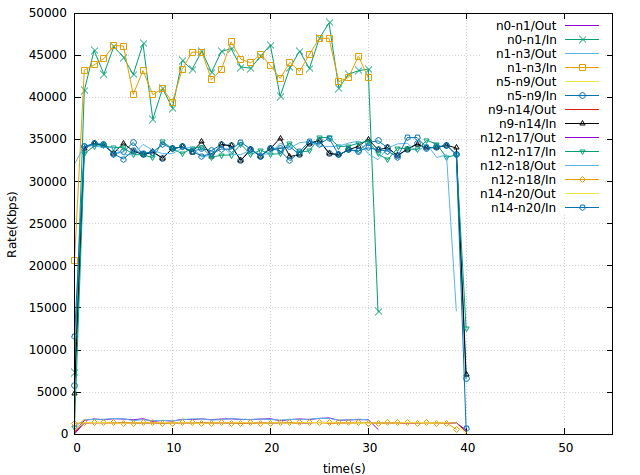
\includegraphics[scale = 0.4]{Figures/step1.png}

\caption{Producer Mobility step 1 (Rate vs Time) Large} \label{step1} 


\end{center}

\end{figure}






\begin{figure}[H]

\begin{center}


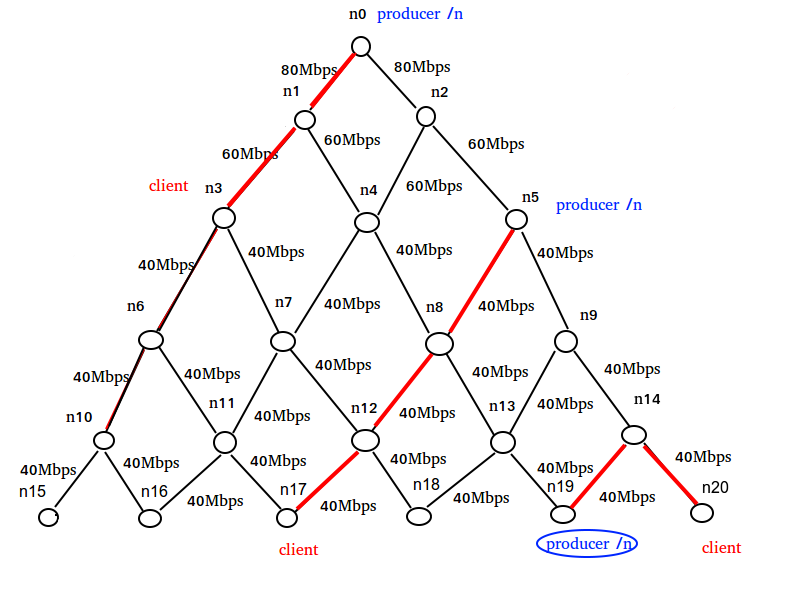
\includegraphics[scale = 0.4]{Figures/Step2.png}

\caption{Producer Mobility step 2 Large} \label{Step2} 

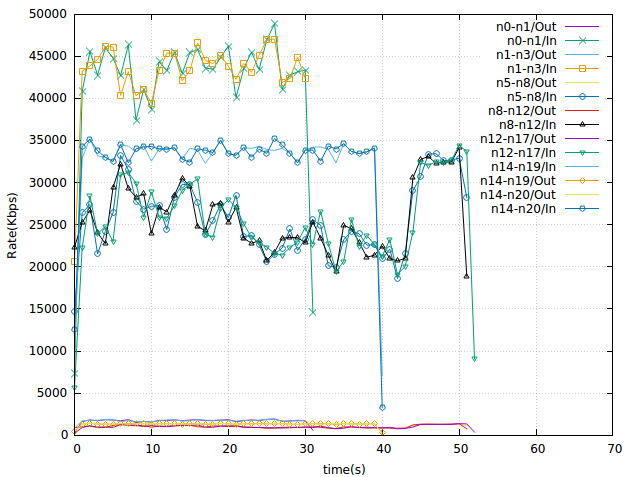
\includegraphics[scale = 0.4]{Figures/step2.png}

\caption{Producer Mobility step 2 (Rate vs Time) Large} \label{step2} 


\end{center}

\end{figure}




\subsection{MaxFlow}
Figure \ref{MaxFlow_big} shows the paths chosen by strategy to maximize the throughput. This strategy works with capacity of each link and according to these value it returns the paths which can maximum the throughput toward clients.

Figure \ref{maxflow_big} shows how the rates are changing during time with this strategy. As you can see data packets have maximum value to achieve the output.  

The mobile stations are connected to $a2,a3$ Access Point can download their contents through taps interfaces.

The algorithm of this strategy is written by finding the paths which maximize throughput with preventing out of range extra loops.

\begin{figure}[H]

\begin{center}

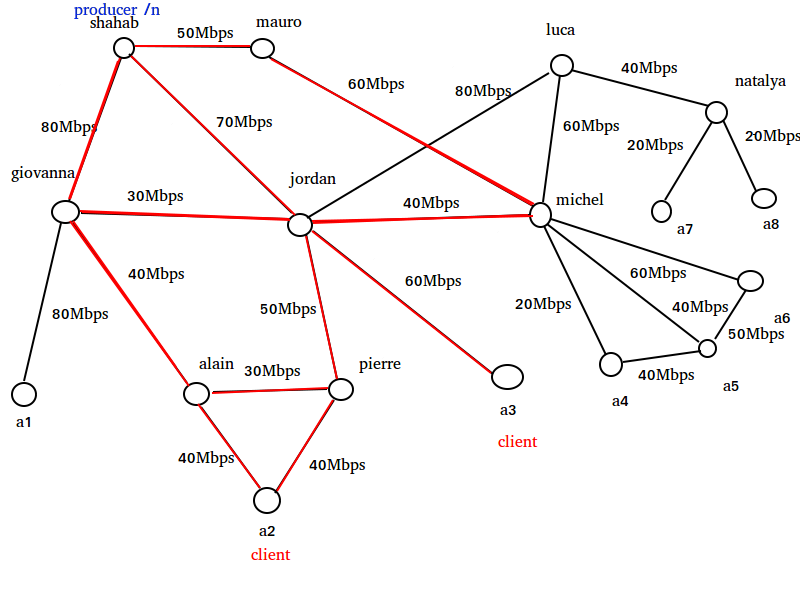
\includegraphics[scale = 0.4]{Figures/MaxFlow_big.png}

\caption{MaxFlow Tree Large} \label{MaxFlow_big} 


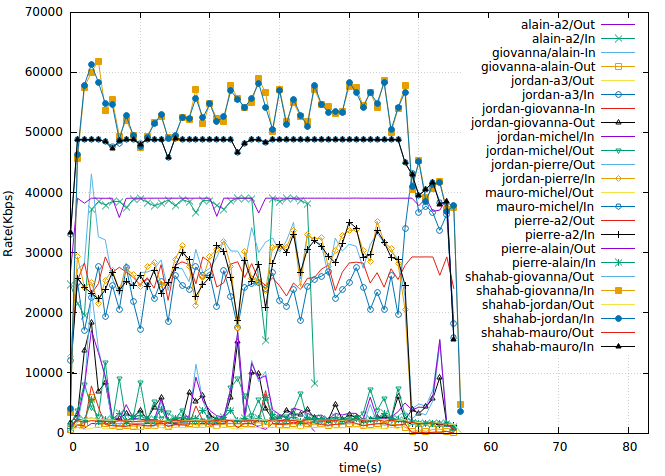
\includegraphics[scale = 0.4]{Figures/maxflow_big.png}

\caption{MaxFlow (Rate vs Time) Large} \label{maxflow_big} 


\end{center}

\end{figure}



